\section{April 25}
Recall that last time, we discussed the quantity \( -(c \Delta t)^2 + (\Delta x)^2 \) and its invariance.
More generally, we can adapt this invariance to include all three dimensions:
\[
	(\Delta s)^2 = -(c \Delta t)^2 + (\Delta x)^2 + (\Delta y)^2 + (\Delta z)^2 = \eta_{\mu \nu}(\Delta
	x)^{\mu}(\Delta x)^{\nu}
\]
and this quantity is usually called the \textit{spacetime interval}. As discussed last time as well, we
require that this quantity be invariant under Lorentz boosts and also spatial rotation. Here, we develop the
formal notation to discuss Lorentz transformations. We've already established that it is a transformation of
some kind, so it's natural to think about a point \( (\Delta x') \) as being derived by multiplying \( (\Delta
x) \) by some matrix \( \Lambda \):
\[
	(\Delta x')^{\mu} = \Lambda^{\mu}_{\nu}(\Delta x)^{\nu}
\]
Then, this notation implies that in the new frame, the spacetime interval is written as:
\[
	\begin{pmatrix} c \Delta t' & \Delta x' & \Delta y' & \Delta z' \end{pmatrix}
	\begin{pmatrix} -1 & & & \\ & 1 & & \\ & & 1 & \\ & & & 1 \end{pmatrix}
	\begin{pmatrix} c \Delta t'\\ \Delta x' \\ \Delta y' \\ \Delta z' \end{pmatrix} = (\Delta x')^{\top}
	\eta (\Delta x') = 
	(\Delta x)^{\sigma}(\Lambda^{\top})^{\rho}_{\sigma} \eta_{\rho \nu} \Lambda^{\mu}_\nu (\Delta x)^{\nu}
\]
\begin{aside}
	Notice that \( (\Delta x')^{\top} \) should be written as a dual vector, but we still write it using an
	upper index \( (\Delta x')^{\top} = (\Delta x)^{\sigma} (\Lambda^{\top})^{\rho}_\sigma \). The reason for
	this is because we want to treat the vector and dual vector on "equal footing", and treat the metric as
	the object such that when we combine the vector and dual together we get a scalar. We will explore this
	more in depth at a later lecture, so keep this in the back of your mind for now.    
\end{aside}

The statement of invariance means we want this to equal \( (\Delta x)^{\sigma} \eta_{\sigma \nu}(\Delta x)^{\nu} \),
so we have the equality:
\[
	(\Delta x)^{\sigma}(\Lambda^{\top})^{\rho}_\sigma \eta_{\rho \mu} \Lambda^{\mu}_{\nu}(\Delta x)^{\nu} =
	(\Delta x)^{\sigma}\eta_{\sigma \nu} (\Delta x)^{\nu}
\]
If we want these two quantities to be the same, then we should require that the Lorentz transformation does
not change the metric. We can see this as \( \Lambda^{\top} \eta \Lambda \) is the "new" metric on the left,
which we require it equal to the one on the right. So, this means we should have the equality: 
\[
	\Lambda^{\top} \eta \Lambda = \eta 
\]
or in index notation,
\[
	(\Lambda^{\top})^{\rho}_{\sigma} \eta_{\rho \nu} \Lambda^{\mu}_\nu = \eta_{\sigma \nu}
\]
Because \( (\Lambda^{\top})^{\rho}_\sigma = \Lambda^{\rho}_\sigma \) (by virtue of transpose) 
then this equation becomes:
\[
	\eta_{\rho \mu}\Lambda^{\rho}_\sigma \Lambda^{\mu}_\nu = \eta_{\sigma \nu}
\]
With this conclusion, we can say that the Lorentz transformation \( \Lambda^{\mu}_\nu \) is one that both
preserves the metric above, and also preserves the handedness (i.e. we want transformations that preserve \(
x \to x \) and not \( x \to -x \)). In terms of the actual form for \( \Lambda \), there are six of them:
\begin{align*}
	\Lambda &= \begin{pmatrix} \cosh \phi & -\sinh \phi & 0 & 0\\ -\sinh \phi & \cosh \phi & 0 & 0\\ 0 &0 & 1
	& 0\\ 0 & 0 & 0 & 1\end{pmatrix}, \quad \begin{pmatrix} \cosh \phi & 0 & -\sinh \phi & 0\\ 0 & 1 & 0 & 0
		\\ -\sinh \phi & 0 & \cosh \phi & 0\\ 0 & 0 & 0 & 1\end{pmatrix}, \quad \begin{pmatrix} \cosh \phi &
	0 & 0 & -\sinh \phi\\ 0 & 1 &0 & 0 \\ 0 & 0 & 1 & 0\\ -\sinh \phi & 0 & 0 & \cosh \phi\end{pmatrix}\\
	\\
		\Lambda &= \begin{pmatrix} \cos \theta & \sin \theta & 0 & 0 \\ -\sin \theta & \cos \theta & 0 & 0 \\
			0  &0 & 1 & 0\\ 0 & 0 & 0 & 1 \end{pmatrix}, \quad \begin{pmatrix} \cos \theta & 0 & \sin \theta
			   & 0 \\ 0 & 1 & 0 & 0 \\ -\sin \theta & 0 & \cos \theta & 0 \\ 0 & 0 & 0 & 1\end{pmatrix}, \quad
			\begin{pmatrix} \cos \theta & 0 & 0 & \sin \theta \\ 0 & 1 &0 & 0\\ 0 & 0 & 1 & 0\\ -\sin \theta
			& 0 & 0 & \cos \theta\end{pmatrix}
\end{align*}
The top row are Lorentz boosts in the \( x, y, z \) directions respectively, and the bottom row are rotations
about the \( z \) axis, \( x \) axis and \( y \) axes, respectively. As for the Lorentz boosts, it's easy to
check that \( (\Delta s')^2 = (\Delta s)^2 \) easily. Firstly, let's write out what the transformed vector
looks like:
\begin{equation}
	\label{lorentz-boost}
	\begin{pmatrix} c \Delta t' \\ \Delta x' \\ \Delta y' \\ \Delta z' \end{pmatrix} = \begin{pmatrix}  \cosh
\phi & -\sinh \phi & & \\ -\sinh \phi & \cosh \phi & & &\\ & & 1 & \\ & & & 1 \end{pmatrix} \begin{pmatrix} c
\Delta t \\ \Delta x \\ \Delta y \\ \Delta z \end{pmatrix}
\end{equation}
So \( (\Delta s')^2 \) is written as:
\begin{align*}
	\begin{split}
	-(c \Delta t')^2 + (\Delta x')^2 &= 
		-\cosh^2 \phi (c \Delta t)^2 - \sinh^2 \phi (\Delta x)^2 + 2 \cosh
		\phi (c \Delta t) \sinh \phi (\Delta x) + \sinh^2 \phi (c \Delta t)^2 \\ &+ \cosh^2 \phi - 2 \cosh \phi \sinh
		\phi (c \Delta t) (\Delta x)
		\end{split}
		\\
		&= [\cosh^2 \phi - \sinh^2 \phi](c \Delta t)^2 + [\cosh^2 \phi - \sinh^2 \phi] (\Delta x)^2
\end{align*}
Then using the identity that \( \cosh^2 \phi - \sinh^2 \phi = 1 \), then \( (\Delta s')^2 = (\Delta s)^2 \),
as required. There is also a physical meaning to this parameter \( \phi \) that we've seemingly mysteriously
introduced, which we can see from the physical interpretation of a Lorentz boost:
\[
	\begin{pmatrix} c \Delta t'\\ \Delta x' \\ \Delta y \\ \Delta z' \end{pmatrix}
	= 
	\begin{pmatrix} \gamma \left( c \Delta t - \frac{v}{c}\Delta x \right)\\ 
	\gamma \left( -\frac{v}{c^2} (c \Delta t) + \Delta x \right)\\
\Delta y \\ 
\Delta z\end{pmatrix}
\]
so comparing this with \cref{lorentz-boost}, we see that:
\[
	\cosh \phi = \gamma \quad \sinh \phi = \frac{\gamma v}{c}
\]
this implies \( \tanh \phi = \frac{\gamma v / c}{\gamma} = v / c \), so \( \phi = \tanh^{-1}(v / c) \). 

\subsection{4-Vectors}
So far in our discussion, the only 4-vector that we've encountered is this quantity \( (\Delta x)^{\mu} \)
that we've been talking about. More generally however, a 4-vector is defined as any vector that transforms in
the same way as \( (\Delta x)^{\mu} \) under a Lorentz transformation. That is:
\[
	V^{\mu} \to V'^{\mu} = \Lambda^{\mu}_\nu V^{\nu}
\]	
Not all \( V \) are valid 4-vectors! Take the following non-example: define \( \tilde u^{\mu} \) as follows:
\[
	\tilde u^{\mu} \equiv \dv{x^{\mu}}{t} = \begin{pmatrix} c \\ u \end{pmatrix}
\]
where \( u^{i} = \dv{x^{i}}{t} \). Then, under a Lorentz boost in the \( x \)-direction, we have:
\[
	\tilde u'^{\mu} = \begin{pmatrix} \dv{(ct')}{t}\\ \dv{x'}{t'} \\ \dv{y'}{t'} \\
	\dv{z'}{t'} \end{pmatrix} = \begin{pmatrix} c \\ \frac{\gamma(dx - v \diff t)}{\gamma
	(\diff t - \frac{v}{c^2} \diff x)}\\ \frac{dy}{\gamma(dt - \frac{v}{c^2} \diff x)} \\
	\frac{dz}{\gamma(dt - \frac{v}{c^2} \diff x)} \end{pmatrix} = 
	\begin{pmatrix} c \\ 
	\\
	\dfrac{u_x - v}{1 - \dfrac{v u_x}{c^2}} \\ 
	\\
	\dfrac{u_y}{\gamma\left( 1 - \dfrac{v u_x}{c^2} \right)}\\ 
	\\
	\dfrac{u_z}{\gamma\left( 1 - \dfrac{v u_x}{c^2} \right)}\end{pmatrix}
\]
The \( x \)-component transforms as:
\[
	u_x \to \frac{u_x - v}{1 - \frac{v u_x}{c^2}}
\]
is the familiar formula for velocity addition in lower division classes. Notice that a transformation like
this is non-linear (this should be obvious), and hence it doesn't transform like \( (\Delta x)^{\mu} \) so it
is not a valid 4-vector. 

As with all vectors, we can define an "inner product" with these vectors, which we define as \( \eta_{\mu
\nu} V^{\mu} W^{\nu} \). This inner product is particularly convenient because it's Lorentz invariant:
\[
	\eta_{\mu \nu}V'^{\mu}W'^{\nu} = \eta_{\mu \nu}\left( \Lambda^{\mu}_\rho V^{\rho} \right)\left(
	\Lambda^{\nu}_\sigma W^{\sigma} \right) = \eta_{\mu \nu} \Lambda^{\mu}_\rho \Lambda^{\nu}_\sigma V^{\rho}
	W^{\sigma} = \eta_{\rho \sigma} V^{\rho}W^{\sigma}
\]
The invariance is nice because it means that regardless of how you Lorentz boost, this is a quantity you can
calculate which is the same in all reference frames. For a particular 4-vector, we define it as space-like,
time-like, or light-like based on its inner product with itself:
\[
	V^2 = \eta_{\mu \nu}V^{\mu}V^{\nu} = \begin{cases}
		< 0 & \text{time-like}\\
		= 0 & \text{light-like} \\ 
		> 0 & \text{space-like}
	\end{cases}
\]
Finally, one last thing which we will take up next lecture: for \( V^{\mu} = (\Delta x)^{\mu} \), we are
constrained by the spacetime interval: \( -(c \Delta t)^2 + (\Delta x)^2 = \text{const.} \), this traces out
the shape of a \textit{hyperbola}! So when we perform a Lorentz transformation, what we essentially do is
move the vector \( (\Delta x)^{\mu} \) along its defined hyperbola, like in the diagram below: 

\begin{center}
	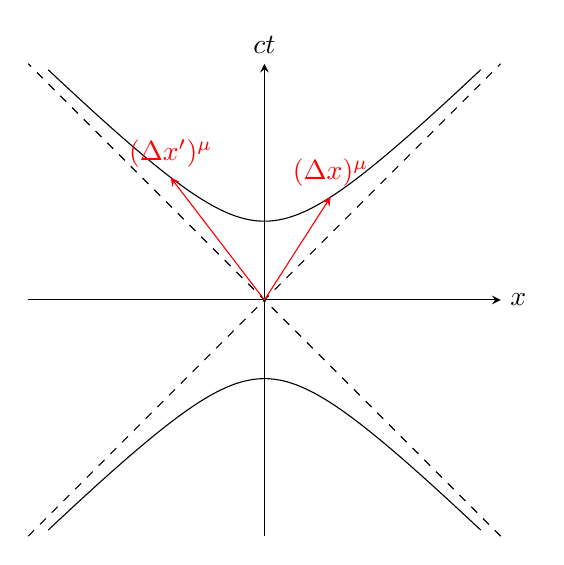
\begin{tikzpicture}
		\draw[-stealth] (-3, 0) -- (3, 0) node[right] {\( x \)};
		\draw[-stealth] (0, -3) -- (0, 3) node[above] {\( ct \)};
		\draw[dashed] (-3, -3 ) -- (3, 3);
		\draw[dashed] (3, -3) -- (-3, 3);
		\draw[rotate around={90:(0, 0)}] plot [variable = \t, samples=1000, domain=-70:70] 
			({1 / cos( \t )}, {1 * tan( \t )});
		\draw[rotate around={90:(0, 0)}] plot [variable = \t, samples=1000, domain=-70:70] 
			({-1 / cos( \t )}, {1 * tan( \t )});
		\draw[-stealth, red, rotate around = {90:(0, 0)}] (0, 0) -- ({1 / cos(-40)}, {1 * tan(-40)})
			node[above=0.2] {\( (\Delta x)^{\mu} \)};
		\draw[-stealth, red, rotate around = {90:(0, 0)}] (0, 0) -- ({1 / cos(50)}, {1 * tan(50)})
			node[above=0.2] {\( (\Delta x')^{\mu} \)};
	\end{tikzpicture}
\end{center}










